\section{Benchmarks}
\label{sec:bench}

We compared our various implementations along two directions: first
we compared the various algorithmic improvements detailed in
\


\subsection{Comparing algorithms in the \haskell implementation}

\begin{figure}[h]
  \centering
  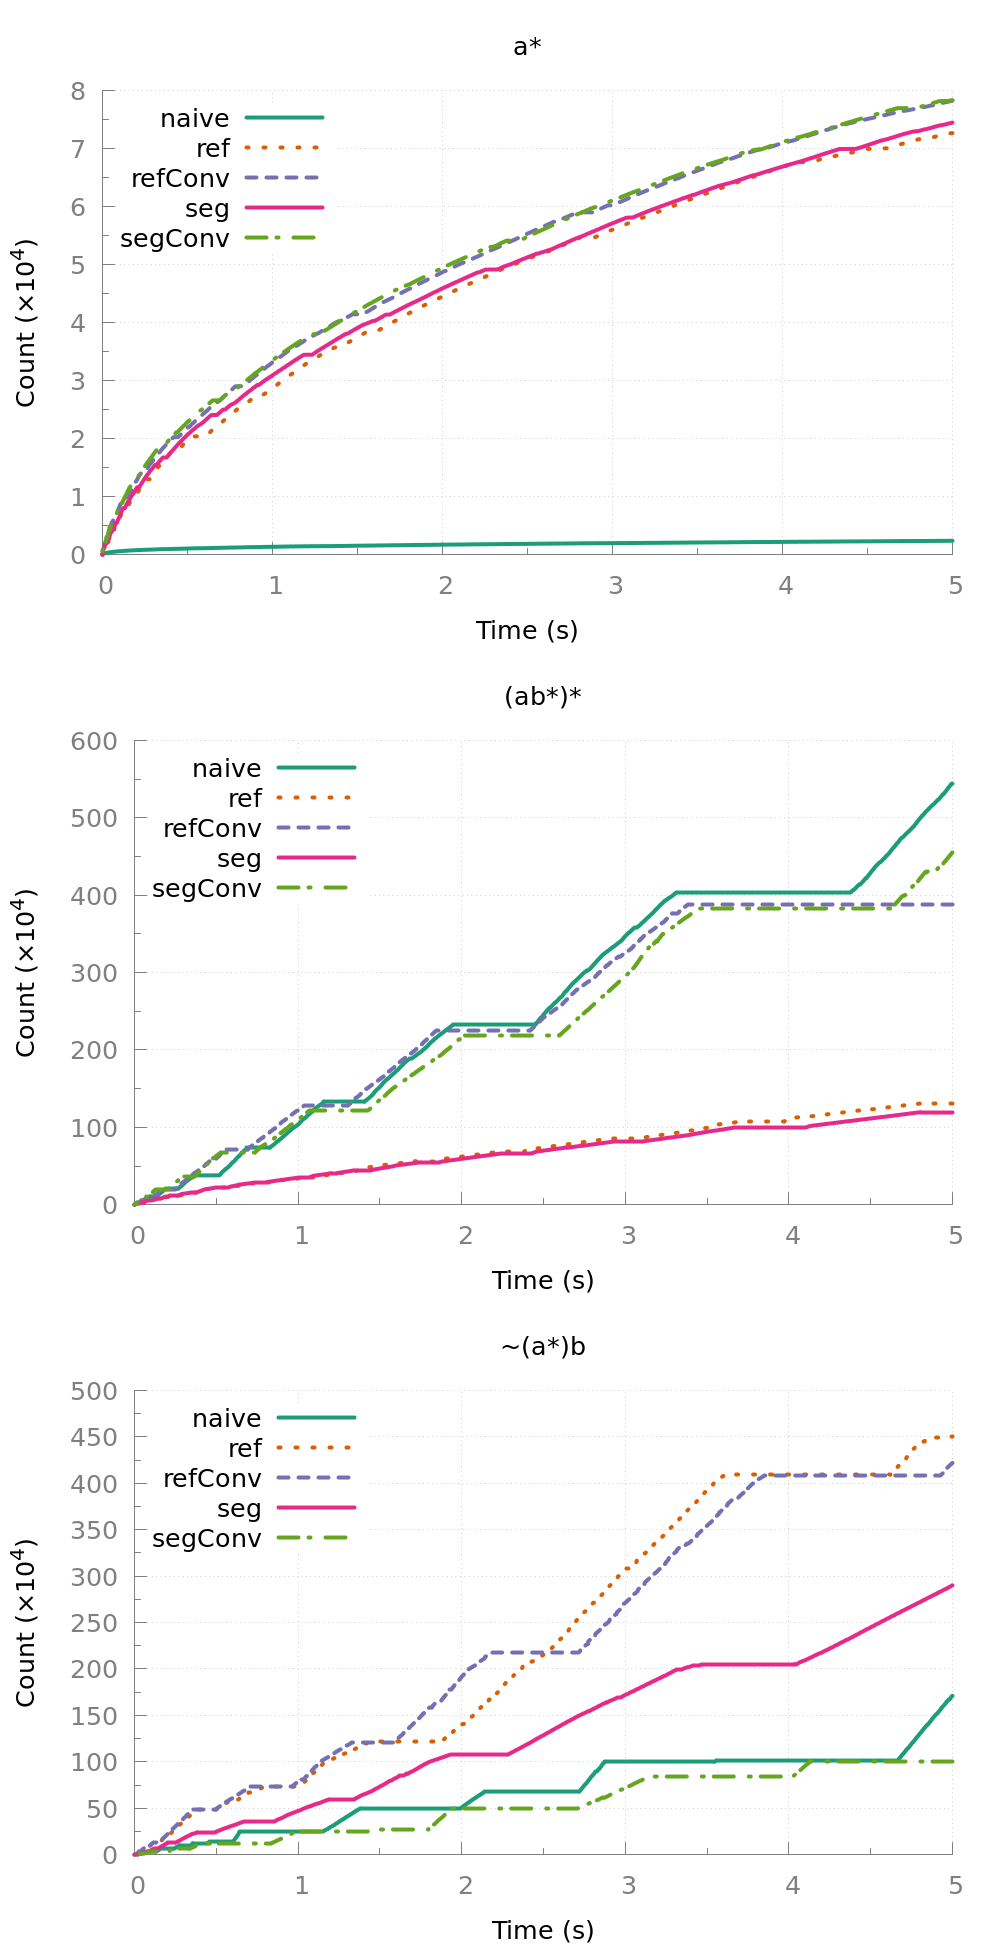
\includegraphics[width=\linewidth]{measure/haskell_all.png}
  \caption{Benchmark for the \haskell implementation with various algorithms}
  \label{bench:haskell:all}
\end{figure}

\subsection{Comparing data-structures in the \ocaml implementation}

We followed the same benchmarking methodology than for the \haskell
version in \autoref{sec:bench}. Benchmark for various data-structures
for regular expressions \verb/a*/, \verb/(ab*)*/ and \verb/~(a*)b/ are
presented in \autoref{bench:ocaml:all}.

\begin{figure}[h]
  \centering
  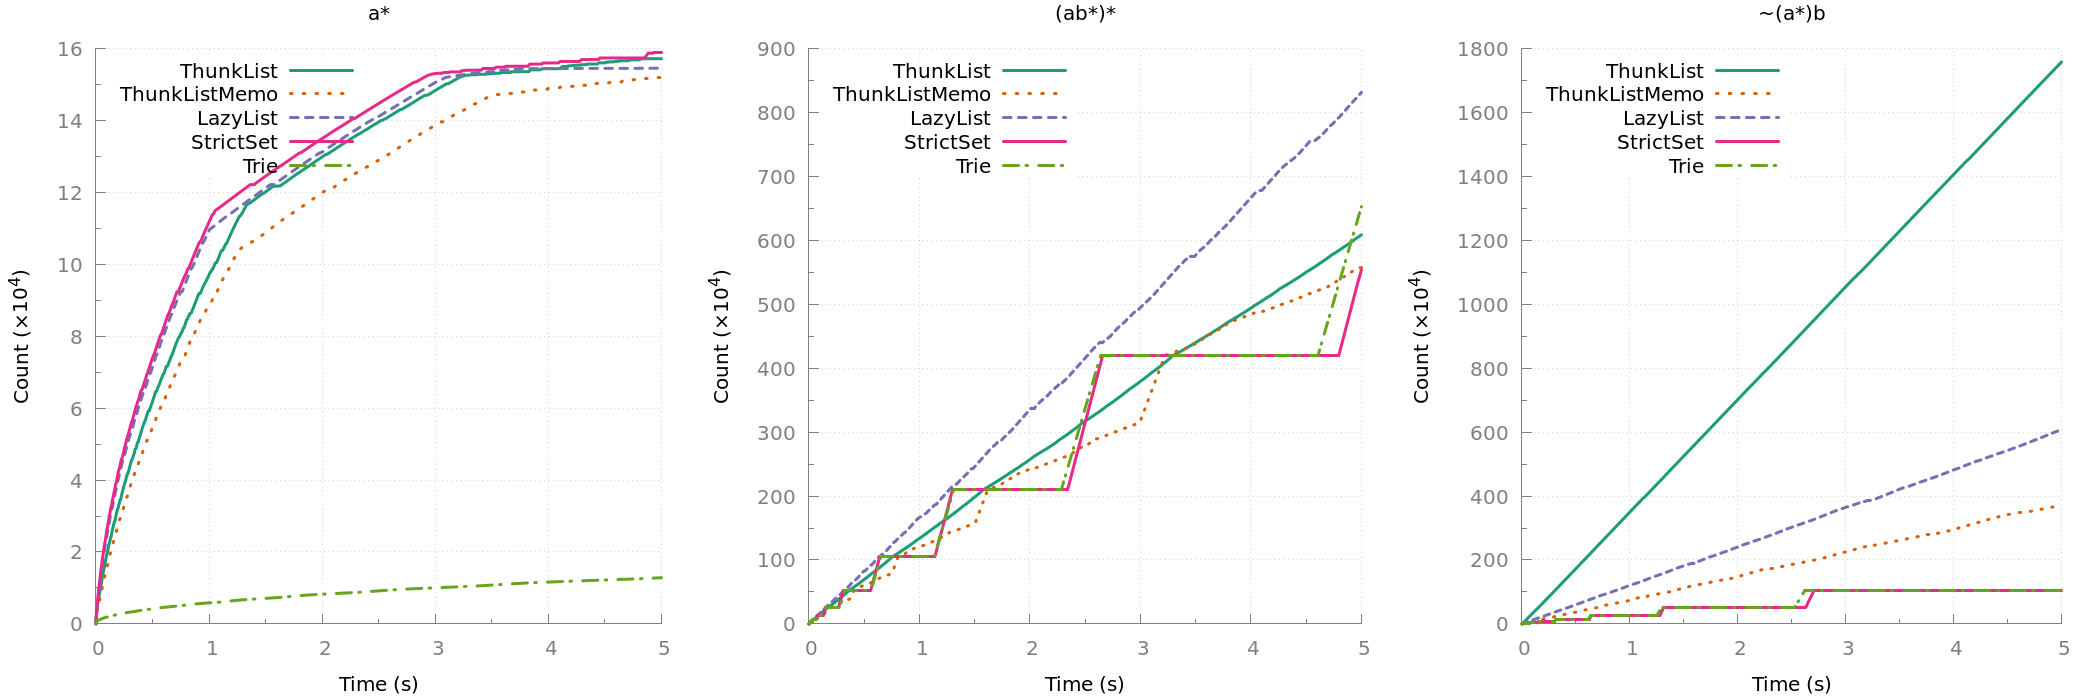
\includegraphics[width=\linewidth]{measure/ocaml_all.png}
  \caption{Benchmark for the \ocaml implementation with various data-structures}
  \label{bench:ocaml:all}
\end{figure}

\subsection{The influence of regular expressions on performances}


\begin{figure}[h]
  \centering
  \begin{subfigure}{0.5\linewidth}
    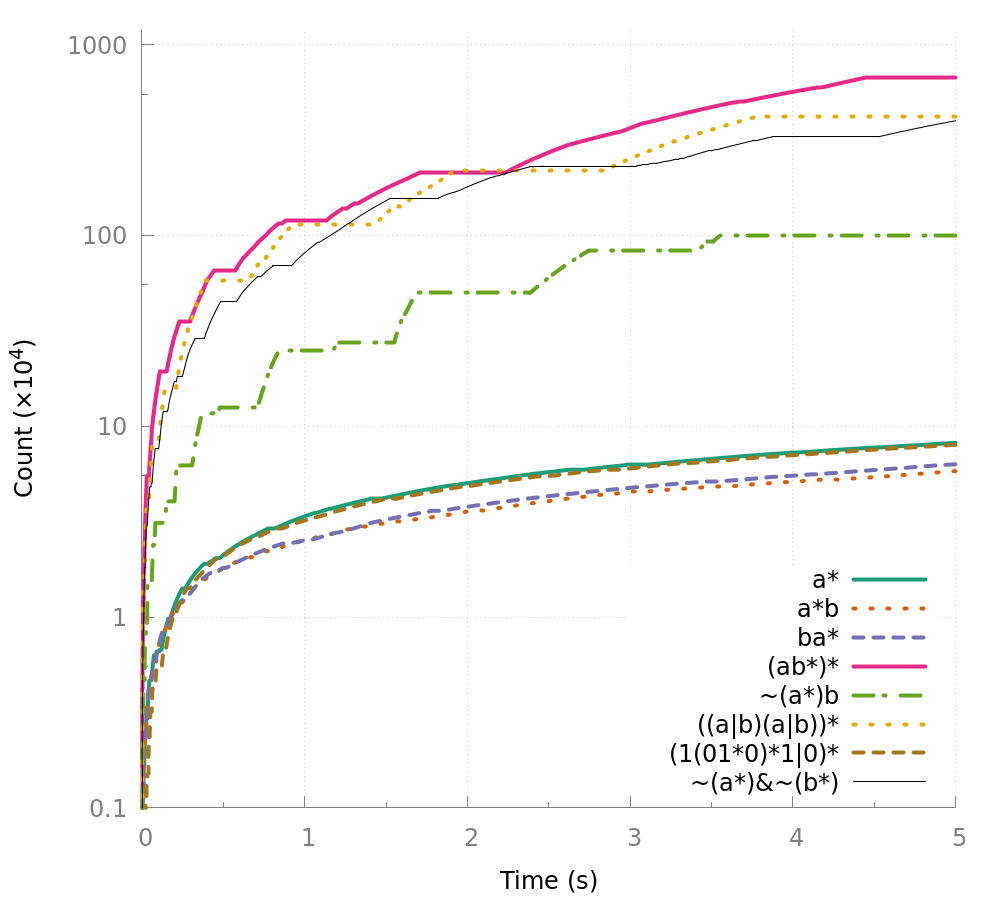
\includegraphics[width=\linewidth]{measure/haskell_langs.png}
    \caption{\haskell implementation with \code{segConv}}
    \label{bench:haskell:langs}
  \end{subfigure}~
  \begin{subfigure}{0.5\linewidth}
    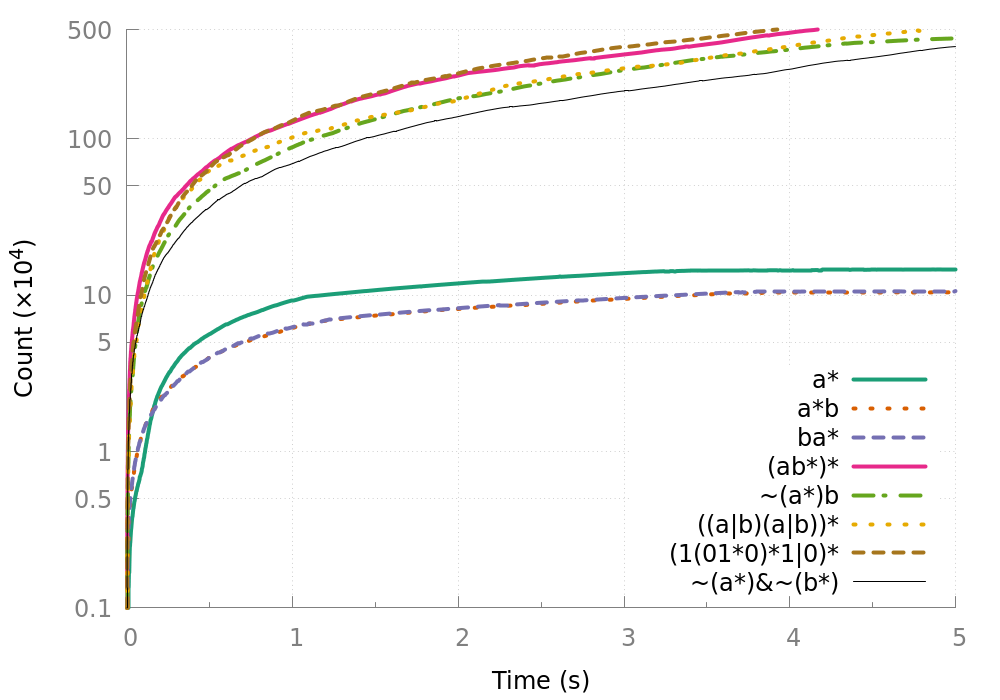
\includegraphics[width=\linewidth]{measure/ocaml_langs.png}
    \caption{\ocaml implementation with \code{ThunkList}}
    \label{bench:ocaml:langs}
  \end{subfigure}
  \caption{Benchmark on different regular expressions}
  \label{bench:langs}
\end{figure}

%%% Local Variables:
%%% mode: latex
%%% TeX-master: "main"
%%% End:
